\begin{frame}{Phân chia miền phụ (Subdomain) theo thiết kế DDD}
\begin{figure}[H]
\centering
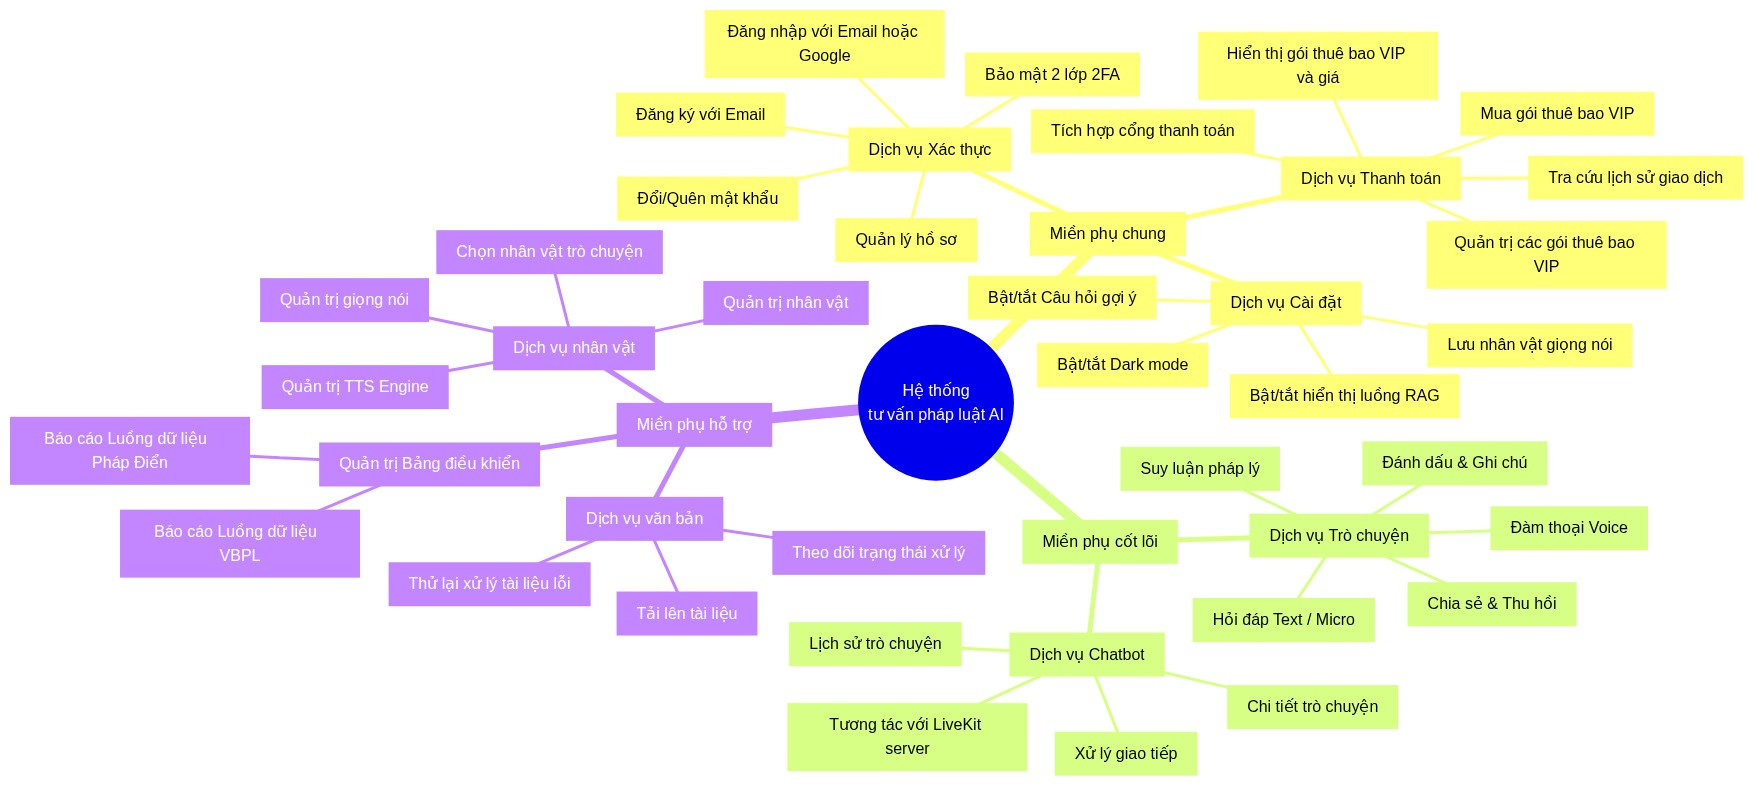
\includegraphics[height=0.55\textheight,width=0.9\textwidth,keepaspectratio]{pictures/SubDomainMindMap.png}
\caption{Sơ đồ tổng quan các miền phụ trong dự án}
\end{figure}

\note{
Áp dụng phương pháp Thiết kế hướng miền (DDD - Domain Driven Design), bài toán lớn của hệ thống được bóc tách và phân chia thành các miền phụ (Subdomain) với mức độ ưu tiên và chức năng riêng biệt.
Chúng ta có Miền phụ cốt lõi (Core Subdomain) tập trung vào nghiệp vụ chính là tư vấn pháp lý và đàm thoại thời gian thực, Miền phụ hỗ trợ (Supporting Subdomain) như quản lý tài liệu, trò chuyện, thanh toán và Miền phụ chung (Generic Subdomain) như xác thực tài khoản.
}
\end{frame}
